\chapter{Entrees}

\section{Scott's Killer Chili\index{entrees!chili}}

\textit{I hope you're prepared for this.  This recipe from Scott
Evans makes a {\em thick} and {\em spicy} chile.  
In the word's of the author ``It is pretty spicy.''  This
is one of those recipes that should include a Disney-style warning label,
``...those with heart conditions or over the age of sixty-five...etc. etc.'' 
This is this recipe's first time in print so some experimentation may be
required.  Supposedly this is a campout recipe, however I see no way that
anyone could possibly carry all these ingredients.  The recipe makes about 16 
servings or less for REALLY big people.  Good luck and here it goes.}
\begin{ingredients}
3 lbs. of hot Italian sausage (ie. Hot Cinncinnati Brand, that homer) \\
3 lbs. bacon \\
3 large onions \\
3 bell peppers (2 green, 1 red) \\
4--5 cloves of garlic \\
4--5 hot peppers (a cornucopiea of jalapenos, habeneros, and others) \\
3 cans Italian pear tomatoes \\
1 Tbsp. olive oil \\
1 Tbsp. mustard powder \\
1 Tbsp. celery seed \\
1 Tbsp. chili powder \\
1 Tbsp. bay leaves \\
1 Tbsp. Worcester sauce \\
1 Tbsp. vinegar \\
red wine \\
water \\
salt and pepper
\end{ingredients}
Start with a large Dutch oven and a campfire right after breadfast.  Fry the
sausage and set aside.  Fry the bacon and set aside.  Leave a bit of grease in
the pot and add the minced garlic followed by the roughly chopped onions and
bell peppers (no bell pepper seeds).  Chop the hot peppers and add to the pot,
remember that the seeds make the dish VERY spicy.  Add olive oil as needed. 
Add about one Tbsp full each of: 
\begin{wrapfigure}{r}{3in}
\centering{
\includegraphics[width=2.8in,clip]{chilli.ps}}
\end{wrapfigure}
mustard powder, celery seed, Worcester
sauce, vinegar, and chili powder.  This may require some experimentation to
alter to your taste.  Stir and cook until onions become clear and peppers begin
to soften.  Add up to one cup of red wine.  Next add tomatos and juices.  Stir
and chop tomatoes.  Add sausage, bacon, and two bay leaves.  Season with salt
and pepper.  Now everything should look a bit like chunky soup, but don't
worry.

Let the chili simmer over low heat for a minimum of three hours, but try for
eight (trust Scott on this one). Check periodically and stir.  If mixture
thickens too much add some water.  Taste and adjust to preference.

Serve with shredded cheddar cheese and garlic bread.  This recipe freezes well
in personalized zip-lock bags (In case you're not hungry enough to eat 
six pounds of meat in one sitting).

\section{Chicken Breasts with Orange Sauce\index{entrees!chicken,
orange sauce}}

\textit{This is a  recipe from Lil and Don Johnson.  Grammie (Lil) passed
it to Martha, who passed it to Kate, and so on, and so on, and so
on... It's good.}
\begin{ingredients}
4 halved chicken breasts \\
1 small can undiluted O.J. concentrate \\
1 package Lipton's Onion Soup Mix \\
paprika
\end{ingredients}
In a long baking pan arrange the 8 pieces of chicken.  Pour the O.J.
concentrate (at room temperature) over the chicken.  Sprinkle the soup mix over
the chicken.  Add a little paprika for seasoning.

Cover pan with foil.  Bake at \oven{350} for 40 minutes.  Remove foil and baste
chicken.  Back for an additional 20 minutes uncovered.

\section{Porcupine Meatballs\index{entrees!meatballs}}

\textit{This is a recipe from Mickey and George, Sr. Evans.}
\begin{ingredients}
1\ 1/2 lbs. hamburger \\
3/4 cup uncooked rice \\
1 tsp. salt \\
1 egg \\
1/2 tsp. pepper \\
1/4 cup chopped onion \\
2\ 1/2 cup stewed tomatoes \\
1 tsp. chili \\
1 tsp. sugar
\end{ingredients}
Combine hamburger, rice, salt, egg, pepper, and onion.  Shape into 1\ 1/2$''$
balls.

Heat sauce and chili to boiling in a kettle.  Drop balls in sauce.  Simmer for
1\ 1/2 hours comvered.  Strips of bacon may be wrapped around meatballs and
secured with toothpicks before cooking in sauce.

\section{Lemon-Herb Chicken\index{entrees!lemon-herb chicken}}

\textit{This is Fermina's favorite.}
\begin{ingredients}
1 chicken (cut) or 3\ 1/2 pounds of chicken parts \\
1/2 cup olive oil \\
1/4 cup lemon juice \\
2 garlic cloves minced \\
3 Tbsp. chopped fresh oregano or 1 Tbsp. dry \\
1/2 tsp. salt \\
1/8 tsp. pepper \\
1 Tbsp. chopped fresh rosemary or 1 tsp. dry \\
2 Tbsp. chopped fresh parsley
\end{ingredients} 
Place chicken meaty side down in a $13''\times 9\times 2''$ baking pan.  
Combine next 8
ingredients, mix well.  Pour mixture over chicken.  Marinate in refrigerator
for two hours.  Bake uncovered at \oven{350} for 40 minutes.  Turn chicken. 
Broil 6'' from heat for 5--10 minutes or until crisp and lightly browned.

\section{Stuffed Flank Steak Teriyaki\index{entrees!flank steak
teriyaki}}

\textit{This belongs because it is MY favorite and since I'm (Tom) 
in charge, well there you go.  Makes 4--5 servings.}
\begin{ingredients}
1 medium to large beef flank steak (1\ 1/4--2 pounds) \\
1/2 cup soy sauce \\
1/4 cup cooking oil \\
2 Tbsp. molasses \\
2 tsp. dry mustard \\
1 tsp. gingeroot or 1/2 tsp. dry ginger \\
1 clove garlic minced \\
1 cup water \\
1/2 cup long-grain rice \\
1/2 cup of shredded carrots \\
1/2 cup sliced water chestnuts (optional) \\
1/4 cup sliced green onions
\end{ingredients}
\begin{wrapfigure}{l}{3in}
\centerline{\includegraphics[width=2.8in,clip]{flank.ps}}
\end{wrapfigure}
Cut a large pocket in flank steak or have your butcher do it.  Combine soy
sauce, oil, molasses, mustard, ginger, and garlic.  Place meat in shallow pan
or plastic bag.  Pour marinade into pocket and over meat. Let stand at room
temp (\oven{300}K) for 30 minutes or in refrigirator for 2--3 hours.

In saucepan combine water, rice, carrots, water chestnuts, and green onion. 
Bring to a boil; reduce heat and simmer while covered for 8 minutes.  Remove
from heat and set aside. 

Drain meat reserving marinade.  Add 1/4 cup of reserved marinade to the rice
mixture.  Spoon rice stuffing into pocket of meat.  Secure end with wooden
toothpicks.  Place meat in shallow roasting pan and cover with foil.  Bake at
\oven{350} for 1 hour until meat is done.

Fermina allows an extra 10--15 minutes without foil to brown meat.  Brush with
marinade while browning and check often.  Slice meat diagonally across grain to
serve.

\section{Better-than-vegetarian Pasta Sauce\index{entrees!better-than-veggie
pasta sauce}}

\textit{This from Kate's brother Don, and he got it from his friend Dawn
Ollila. The honey/brown sugar and cinnamon addition is what makes it taste so
special}.
\begin{ingredients}
1 Tbsp. olive oil \\
1 onion \\
1 green pepper \\
2 cloves of minced garlic \\
1 tomato\\
1 large or two small carrots OR 1/4 cup cup lentil beans \\
1 or 2 cans of tomato sauce \\
thyme \\
basil \\
oregano \\
rosemary \\
1 Tbsp. honey or brown sugar \\
cinnamon \\
salt and pepper \\
\end{ingredients}
Saute the 4 vegetables in olive oil, adding them as ordered above. When the
onion is clear and the tomato is soft, add the tomato sauce.  Bring to a
simmer. The sauce is now tasty, but to thin to stick to the pasta.
Choose either the carrots or lentils to give it body. Lentils add a great dark,
almost meaty, flavor but you will need to boil them in 4 times their
measurement in boiling water for 45 minutes to 1 1/2 hours first (no presoaking
required). Do not add them to the sauce until they are bean-like mush. or, you
can grate the carrot as finely as you have the technology to do and add to
the sauce. The taste is minimal, but the texture is great. Add the rest of the
ingredients and adjust to taste. Add just enough cinnamon to make your guests
look at you funny and say, ``What did you put in this?'' The flavor actually
works quite well.

\section{Peachy Chicken\index{entrees!peachy chicken}}

\textit{From Fermi, this is Betsy's favorite.  Tom:  Actually I
really don't like this recipe and the only reason she ``likes'' this one is
because she hates my favorite recipe (stuffed flank steak).  Note:  the
``peachy'' in ``peachy chicken'' is not a southern thing.  Kate:  When Tom and
I were first married (Tom interjects: forty years ago) I made a chicken dish
with fruit.  He honestly thought I was trying to annoy him (how did he know?).}
\begin{ingredients}
chicken parts for 4--6 people\\
1 large can peach halves (drained, reserve syrup)\\
2 Tbsp. soy sauce\\
2 Tbsp. lemon juice\\
1/2 Tbsp. ginger\\
2 cloves minced garlic
\end{ingredients}
Preheat oven to \oven{375}.  Mix last four ingredients with reserved peach
syrup.  Pour marinade over chicken parts in roasting or baking pan. Bake in
oven for 45--60 minutes. Turn once.  Add peach halves last 15 minutes.  Brown
under broiler for a few minutes if further browning is needed.

\centerline{
\includegraphics[scale=.5,clip]{meatloaf.ps}}

\section{Swiss Meatloaf\index{entrees!swiss meatloaf}}
\label{sec:swiss-meatloaf}

\textit{This was contributed by Joyce Evans, and is definitely ``comfort
food''! Serves 6.}
\begin{ingredients}
1 egg \\
1/2 cup evaporated milk \\
1 tsp. rubbed sage \\
1 tsp. salt \\
1/2 tsp. black pepper \\
1 1/2 lbs. lean ground beef \\
1 cup cracker crumbs (round buttery type, approx. 24) \\
3/4 cup grated Swiss cheese \\
1/4 cup finely chopped onion \\
2-3 strips bacon, cut into 1 in. pieces \\
\end{ingredients}
Preheat oven to \oven{350}. Beat the egg in a large bowl. Add evaporated milk, 
sage, salt, and pepper.  Mix together. Add beef, crumbs, 1/2 cup of the cheese
and the onion. Blend. Form into a loaf and place in a 2 quart rectangular dish.
Arrange bacon pieces on top of the loaf, and bake for 40 minutes. Sprinkle
remaining 1/4 cup cheese on top and bake 40 minutes longer. 

\section{Devilled Crabs\index{entrees!devilled crabs}}

\textit{This is from Dodge and Martha Johnson in memory of
a great southern cook, Martha Hodgkins Niepold Lamb (Kate's Grandmother).
Don't be scared by the lack of ingredient quantities. Its easy and delicious.
Just adjust until it tastes good.}
\begin{ingredients}
1 stick butter\\
2 eggs\\
a little flour and water\\
Worchestershire sauce\\
dry mustard\\
vinegar\\
pinch of sugar, salt, pepper, and MSG\\
1 lb. crab
\end{ingredients}
Preheat oven to \oven{350}.  Melt butter. Mix eggs with flour and water and add
to butter. Continue mixing and add everything else. stuff in scallop shells or
small casseroles and dot with butter and bread crumbs. Bake for 1 hour.
\begin{center}
    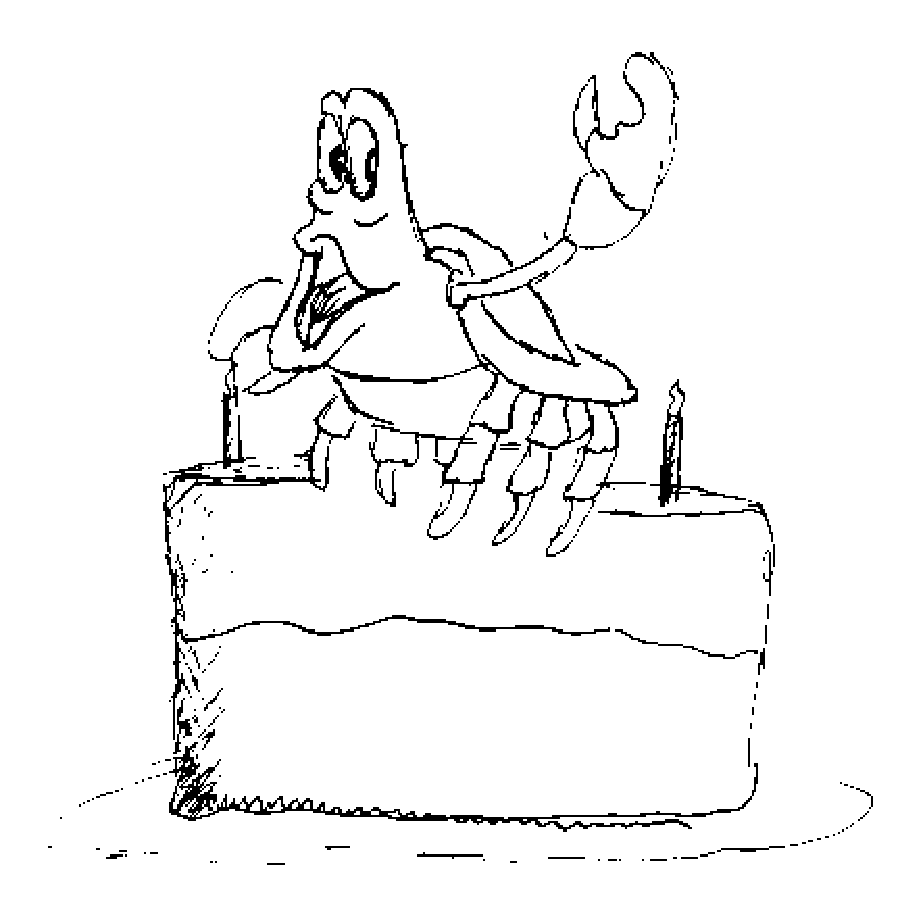
\includegraphics[width=3in,clip]{crab.ps}
\end{center}

\section{Orange Game Hens\index{entrees!Orange Game Hens}}

\textit{This is a recipe courtesy of Martha and Dodge Johnson's friends, the
Nicolsons. It's a great dish for company-especially at their house because
they are such nice people and good cooks!}
\begin{ingredients}
2 or more Cornish game hens, whole or halved\\
Joyce Chen's orange Szechuan sauce (or sub in soy sauce with orange 
concentrate)\\
2--3 Tbsp. of orange concentrate\\
several Tbsp. white wine\\
garlic powder\\
ground ginger (fresh or frozen root is best)
\end{ingredients}
Preheat oven to \oven{350}. Pour sauce, concentrate, and wine over hens. Sprinkle
with garlic powder and ginger. Cover and bake for 1 hour, and uncover last 10
minutes. Good over a bed of rice. 

\section{Chapel Hill Chicken Pie\index{entrees!Chapel Hill Chicken Pie}}

\textit{This is from Martha and Dodge, and Kate. Kate's  addition is 
only the
rosemary and measured amounts, for convenience (and my subtractions are those
nasty onions) No one cares what or how mcuh you put in, as long as you are happy.
This is one of those recipes that you put some in, then you take some out (Nana,
does this sound familiar?) This is also the kind of recipe where you vary it
based on what you like or what's sitting in the fridge! It's best when you have
leftover gravy along with meat from a past meal.}
\begin{ingredients}
2 cups chopped meat (roast lamb, beef, or chicken)\\
3--4 cubed and peeled potatoes\\
1.5--2 cups gravy or combination of stock and wine\\
2 Tbsp. flour\\ 
1 tsp. salt\\
2 tsp. pepper\\
1 Tbsp. dried parsley\\
1 tsp. garlic powder or 1 garlic clove\\
1 tsp. thyme (if using chicken or beef)\\
1 Tbsp. fresh rosemary \\
1 tsp. marjoram (if using lamb)\\
1 tsp. tarragon (if using chicken)\\
Pie Crust (\corp{Betty Crocker's} mix is good, sorry 
\corp{Duncan Hines}, you don't make one!) 
\end{ingredients}
1--2 cups each of your favorite vegetables, such as  
\begin{ingredients}
chopped carrots\\ 
green beans\\
celery\\ 
onion\\
mushrooms\\
peas\\
\end{ingredients}
Preheat oven to \oven{450}. Boil potatoes until somewhat cooked through, about
15 minutes. In a flat-ish casserole (1.5-2 qt.), layer meat, vegetables, and
potatoes. sprinlke spices over, and then flour. Add gravy mixture; adjust so
the liquid comes up about half the height of the ingredients.  Top with crust,
seal edges, and add fork holes or vents. Brown for 15 minutes, then then lower
temperature to \oven{350} and bake for 45 minutes longer. I find that I have to
cover it for the last 15 minutes or so to keep the crust from getting too brown.

\section{Pasta with Prosciutto\index{entrees!Pasta with Prosciutto}}

\textit{Martha and Dodge originally got this from the New York Times,
but it has evolved. It's
rather quick and satisfying. They say the order of tasks is a little tricky for
non-Italian cooks. Luckily, half the family  need not worry.}
\begin{ingredients}
3 cups chopped plum tomatoes\\
2-3 thinly sliced small zucchini\\
1/8-1/4 lb. prosciutto, cut into strips\\
1 tsp. salt\\
2 tsp. pepper\\
1/2 tsp. red pepper flakes (optional)\\
1 cup whipping cream
1/2 cup chopped fresh basil\\
1/4 cup grated parmesam (use the real thing not the cylinder, people)\\
1+ cloves garlic, chopped\\
1 Tbsp. olive oil\\
about 3/4 lb. pasta 
\end{ingredients}
Cook pasta. Save 1/3 cup cooking water. In frying pan, sear garlic, add
zucchini, prosciutto, salt and pepper, red pepper flakes, then tomatoes.
Stir for 2-3 minutes.  Add saved water, cream and simmer briefly. Add
pasta, basil, and parmesan, and toss. Transfer to serving dish and eat
immediately (not difficult to do!) Serves 2-3.

\section{Pasta al Cavalfiore (with Cauliflower)
\index{entrees!Pasta al Cavalfiore}}

\textit{Don sends this yummy looking dish from the Moosewood cookbook. Don says
it's good and adds ``so enough of sending pasta recipes to the Italians.''}
\begin{ingredients}
1 onion (optional if you're Kate)\\
1 cauliflower head, chopped into bite sizes\\
1 tomato\\
garlic to taste\\
2 cups grated cheese (see below)\\
1/4 cup olive oil\\
1 can tomato sauce\\
3/4 lb. pasta\\
basil, dried and some fresh too if possible\\
1 tsp. salt\\
1 tsp. pepper
\end{ingredients}
Chop the onion and garlic and saute them in 1 Tsp oil with the basil. When
onion is clear, add cauliflower and cook until tender. (Don tip: add a
handful of water, and cover to speed this along.) Add chopped tomato,
tomato sauce, salt and pepper, and simmer for about twenty minutes. During
this time, cook and drain pasta. Add the remaining olive oil to pasta
along with fresh basil and half the cheese. Don recommends the cheese be
a mixture of parmesan, romano, mozzarella, and cheddar. Spread this on a big
platter and top with the cauliflower mixture. Top with remaining cheese. Don
recommends a California gewurtstraminer ``to go with.''  Serves 2-3.

\section{Sweet and Sour Pork\index{entrees!Sweet and Sour Pork}}

\textit{Tom and Kate eat this a lot; its a ``regular''. It's 
word-for-word from a Southern Living year-end cookbook I
love (1992, if curious). Its quite delicious, and its even somewhat 
healthy.}
\begin{ingredients}
1 Tbsp. sherry\\
1 Tbsp. soy sauce\\
1 Tbsp. cornstarch\\
1 lb boneless pork, cut into cubes\\
1/4 vegetable oil, divided\\
1 clove garlic, minced\\
1 small onion (optional)\\
2 green peppers, cut into 1 in. pieces\\
1/3 cup sugar\\
1/4 cup ketchup\\\
1 Tbsp. sherry\\
2 Tbsp. soy sauce\\
2 Tbsp. white vinegar\\
1 Tbsp. cornstarch\\
1/3 cup water\\
1 8 oz. can pineapple slices in juice, each cut into about 8 pieces
\end{ingredients}
Combine first 3 ingredients, add pork, and let marinate 20 minutes (or however
long it takes to prepare everything else). Heat 2 Tbsp. oil in big frying pan.
Stir fry onion garlic, and green pepper over med-high heat until crisp tender.
Remove from skillet. Add rest of oil and cook pork until cooked through.
Stir in cooked vegetables. Combine sugar and next 6 ingredients, stirring
until cornstarch dissolves. Add to pork mixture and cook until it comes to
a boil. Add pineapple and and boil for about 1 minute. Serve over hot
cooked rice. Serves 2-3 hungry people.
